% Created 2022-11-25 vie 12:23
% Intended LaTeX compiler: pdflatex
\documentclass[10pt]{article}
\usepackage[utf8]{inputenc}
\usepackage[T1]{fontenc}
\usepackage{graphicx}
\usepackage{grffile}
\usepackage{longtable}
\usepackage{wrapfig}
\usepackage{rotating}
\usepackage[normalem]{ulem}
\usepackage{amsmath}
\usepackage{textcomp}
\usepackage{amssymb}
\usepackage{capt-of}
\usepackage{hyperref}
\usepackage[spanish]{babel}
\usepackage{graphicx,geometry}
\geometry{ a4paper, left=1in, right=1in, top=1in, bottom=1in }
\renewcommand\familydefault{\sfdefault}
\usepackage{sectsty}
\sectionfont{\normalfont\Large }
\subsectionfont{\normalfont}
\usepackage{tabularx}
\usepackage{listings}
\lstdefinestyle{mystyle}{
basicstyle=\ttfamily\footnotesize,
numbers=left,
showspaces=false,
frame=single,
showspaces=false,
showstringspaces=false,
showtabs=false,
numberstyle=\tiny,
aboveskip=\parskip
}
\lstset{
style=mystyle,
literate={á}{{\'a}}1
{é}{{\'e}}1
{í}{{\'{\i}}}1
{ó}{{\'o}}1
{ú}{{\'u}}1
{Á}{{\'A}}1
{É}{{\'E}}1
{Í}{{\'I}}1
{Ó}{{\'O}}1
{Ú}{{\'U}}1
{ü}{{\"u}}1
{Ü}{{\"U}}1
{ñ}{{\~n}}1
{Ñ}{{\~N}}1
{¿}{{?``}}1
{¡}{{!``}}1
}
\makeatletter
\usepackage{fancyhdr}
\pagestyle{fancy}
\usepackage{mdframed}
\BeforeBeginEnvironment{minted}{\begin{mdframed}}
\AfterEndEnvironment{minted}{\end{mdframed}}
\author{Luis Eduardo Galindo Amaya (1274895)}
\date{25-11-2022}
\title{Acceso a subrutinas de ensamblador por \\
programas de alto nivel}
\hypersetup{
 pdfauthor={Luis Eduardo Galindo Amaya (1274895)},
 pdftitle={Acceso a subrutinas de ensamblador por \\
programas de alto nivel},
 pdfkeywords={},
 pdfsubject={},
 pdfcreator={Emacs 26.3 (Org mode 9.1.9)}, 
 pdflang={Spanish}}
\begin{document}



\newcommand{\docente}{Arturo Arreola Alvarez}
\newcommand{\asignatura}{Organización de Computadoras (331)}
\newcommand{\semestre}{2022-2}

\newcommand{\miportada}[1]{
	\begin{titlepage}
		\vspace*{0.75in}
		\begin{flushleft}
			\sffamily
			\large #1       \\
			\Huge 
            \@title         \\
			\hrulefill
			\vspace{0.25in} \\
			\Large \@author \\
			\vspace*{\fill}
            
\includegraphics[width=\textwidth]{../includes/filler.png} \\
			\vspace*{\fill}
			\large
			\begin{tabular}{|l|l|}
              \hline
			  Asignatura & \asignatura \\
			  Docente    & \docente    \\
			  Fecha      & \@date      \\
              \hline
			\end{tabular}
		\end{flushleft}
	\end{titlepage}
}

\miportada{ Práctica 13 }

\fancyhf{}
\lhead{ \asignatura }
\rhead{ \semestre }
\rfoot{Página \thepage}

\setlength\parindent{0pt}   % eliminar el intentado
\setlength{\parskip}{1.2em}
\maketitle

\section*{Objetivo}
\label{sec:org58bfd2f}

Desarrollar subrutinas de lenguaje ensamblador para ser llamadas desde un lenguaje de alto nivel para comprender las convenciones que los compiladores trabajan en sistemas basados en microprocesador.

\section*{Desarrollo}
\label{sec:org171a129}
\subsection*{1. Cree una carpeta llamada P13\_nombre\_apellido. Dentro de esta carpeta crear los archivos \texttt{P13\_c.c} y \texttt{P13\_a.asm}.}
\label{sec:org6f4439c}


\subsection*{2. En el archivo P13\_c.c definir una función externa llamada sumaMatrices, de la siguiente manera:}
\label{sec:org3b44888}

\begin{verbatim}
extern void sumaMatrices(int[WIDTH][HEIGHT], int[WIDTH][HEIGHT],
                         int[WIDTH][HEIGHT], int, int);
\end{verbatim}

\begin{itemize}
\item a. Recibe 5 parámetros, 3 matrices, y otros 2 datos que representan las dimensiones de dichas matrices (Las matrices serán del mismo tamaño).

\item b. Los primeros 2 parámetros son las matrices a ser sumadas. El tercer parámetro es la matriz resultante.

\item c. Crear dos matrices de enteros con las dimensiones WIDTH y HEIGHT. Definir WIDTH y HEIGHT como Macros de C.

\item d. Inicializar ambas matrices.
\end{itemize}


\subsection*{3. En el archivo P13\_a.asm crear la subrutina sumaMatrices que realice el proceso de la suma de todos los elementos de las matrices pasadas como parámetros y los retorne.}
\label{sec:org6af8962}


\subsection*{4. Llamar la subrutina sumaMatrices definida en ensamblador desde C, pasando como parámetros las matrices declaradas anteriormente.}
\label{sec:orgbfecc9f}


\subsection*{5. Validar su algoritmo en ensamblador imprimiendo las matrices desde C.}
\label{sec:org7df1f4a}



\section*{Capturas}
\label{sec:org3265490}
\begin{figure}[htbp]
\centering
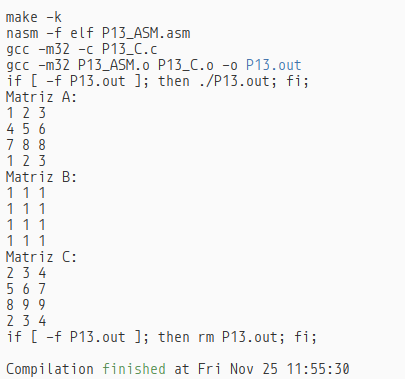
\includegraphics[width=8cm]{src/salida.png}
\caption{Los resultados de la suma estan en la matriz C}
\end{figure}

\section*{Conclusiones y comentarios}
\label{sec:org70de80b}
A pesar de que los lenguajes de alto nivel son muy practicos para implementar algoritmos más complejos hay algunas situaciones en las que la velocidad de ensamblador es muy util, podriamos pensar que tener uno nos hace perder todas las ventajas del otro pero en los lenguajes de bajo nivel es posible integrarlos, solo tenemos que tener cudado con como el programa maneja las variables a basjo nivel.

\pagebreak

\section*{Código}
\label{sec:org9e19f19}
\subsection*{Makefile}
\label{sec:org0c6ea52}
\\ \lstinputlisting{./src/makefile}

\subsection*{P13\_ASM.asm}
\label{sec:org0a051fd}
\\ \lstinputlisting{./src/P13_ASM.asm}

\subsection*{P13\_C.c}
\label{sec:org5c39983}
\\ \lstinputlisting{./src/P13_C.c}
\end{document}
